
\chapter{Introduction}

\section{History of infectious disease}

Infectious diseases have a profound impact on humankind, influencing the course of wars and fates of nations. Only two centuries ago, infectious diseases were the defining challenge of the human condition. For perspective, consider that George Washington was born in 1732, a time when there was no well-defined concept of infection or immunity, no vaccines, and effective treatments for infectious diseases. Washinton suffered from smallpox and multiple debilitating bouts of malaria, suffered wound infections and abscesses, nursed his brother on a tropical island as he died of tuberculosis, and had an influenza pandemic named after him \cite{Fauci:2012us}. Indeed, almost all the major advances in understanding and controlling infectious diseases have occurred in the past two centuries since the founding of the United States. 

The first animal-transmission studies were conducted soon after the War of 1812 and were followed by the development of microscopes, which linked micro-organisms to skin and mucosal diseases. Koch developed a unifying principle of infectious diseases in the late 1800s, proving  four criteria designed to establish a causative relationship between a microbe and a disease. In the early 20\text{th} century Paul Ehrlich developed anti-infective serums and chemicals to destroy pathogens, which paved the way for vaccines, antibiotics, and antiviral agents that have saved hundreds of millions of lives and greatly extended the human life span.

\section{Technology}

\subsection{Historical}

Since the seminal contrabutions of scientists like Koch and Ehrlich, technology has driven our understanding of infectious disease. In 1980, only 1800 validated bacterial species had been published. A  cornerstone of microbiology since the nineteenth century, cultivation \emph{in vitro} fails for many microbes that have adapted to niches that are not easily recalculated in laboratory culture. With this in mind, the advent of DNA-based analyses enable direct identification of micro-organisms by directly reading regions of DNA or RNA genome and performing taxonomy based upon this digital signature. Hantavirus pulmonary syndrome, an ancient disease caused by a phlebovirus, was discovered unexpectedly in 1993 by the application polymerase chain reaction (PCR). Less than a year later, PCR-related subtraction techniques solved a century-old mystery of the cause of Kaposi\' s sarcoma, human herpesvirus 8. Since that time, DNA-based analyses have become far cheaper and are now accelerating the discovery of microorganisms (Figure ~\ref{fig:Fig1}) \cite{Fournier:2013ew}.

\begin{figure*}
\center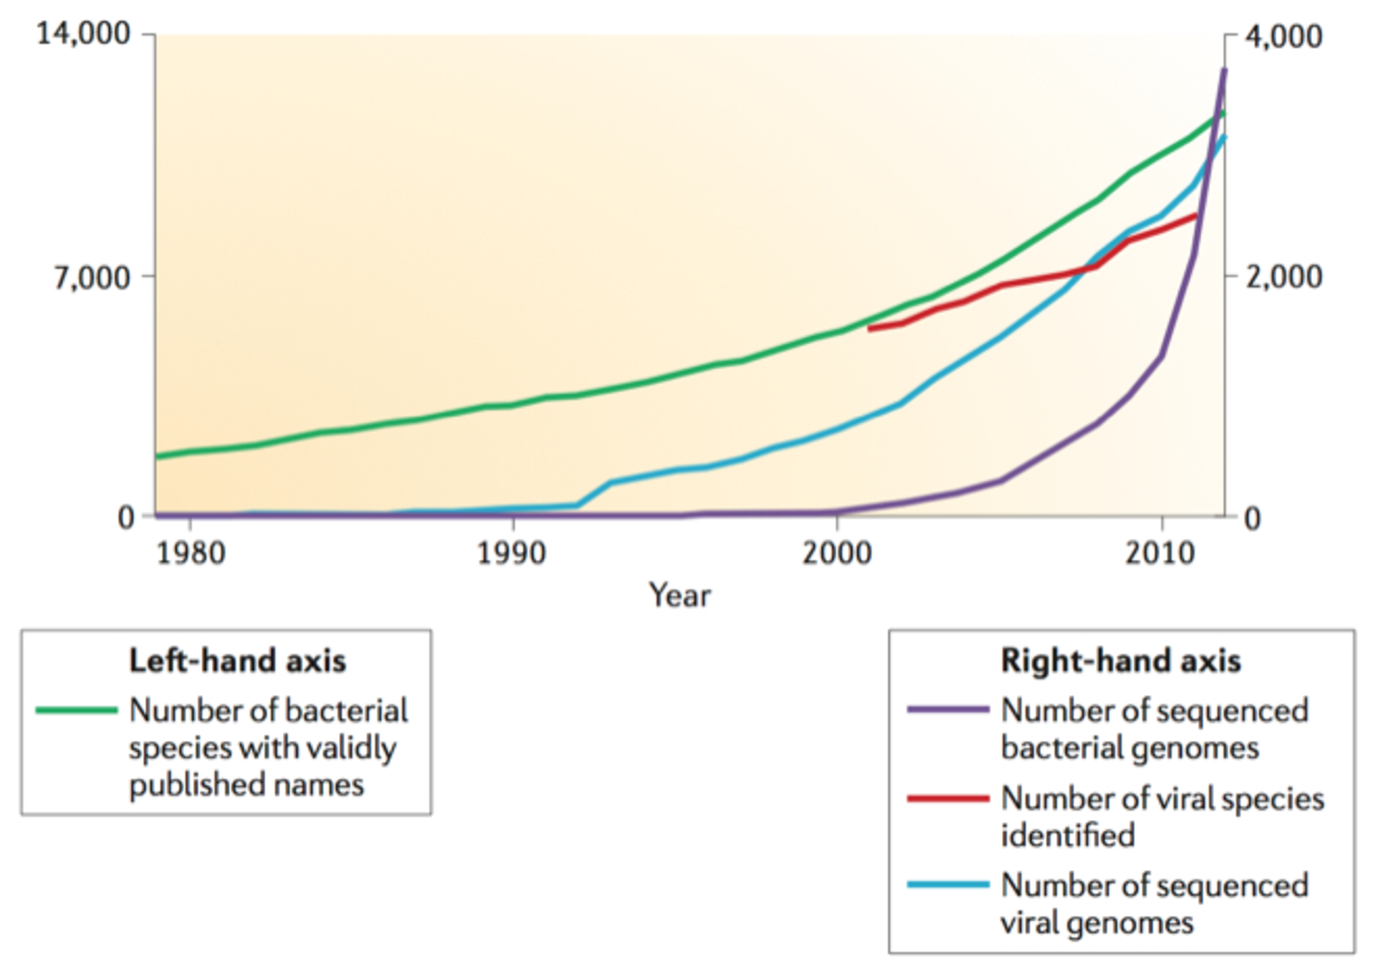
\includegraphics[width=120mm,scale=0.5]{Figures/Fig1}
\caption{Rapid growth in the identification of micro-organisms.}
\label{fig:Fig1}
\end{figure*}

Unlike many chronic and lifestyle-associated diseases resulting from multiple, interacting risk cofactors, most infectious diseases are caused by a single agent. Identification typically points the way not only to general disease-control measures (e.g., sanitation, chemical disinfection, hand washing, or vector control) but also to specific treatment (e.g., vaccination or antimicrobial treatment) \cite{Fauci:2012us}. In turn, tools to rapidly identify the causative agent for a presented infection have been widely sought and developed. The challenge has historically been a trade-off between resolution scope. Whereas laboratory culture methods have reasonable scope (e.g., many organisms can grow and be identified via culture-based methods), the resolution is often poor. It often provides no way to distinguish between strain or species. Furthermore, many microorganisms do not effective grow in culture conditions. On the other hand, DNA-based methods such as qPCR have high resolution (e.g., very specifically identify a single microorganism) but only have a single target.

\begin{figure*}
\center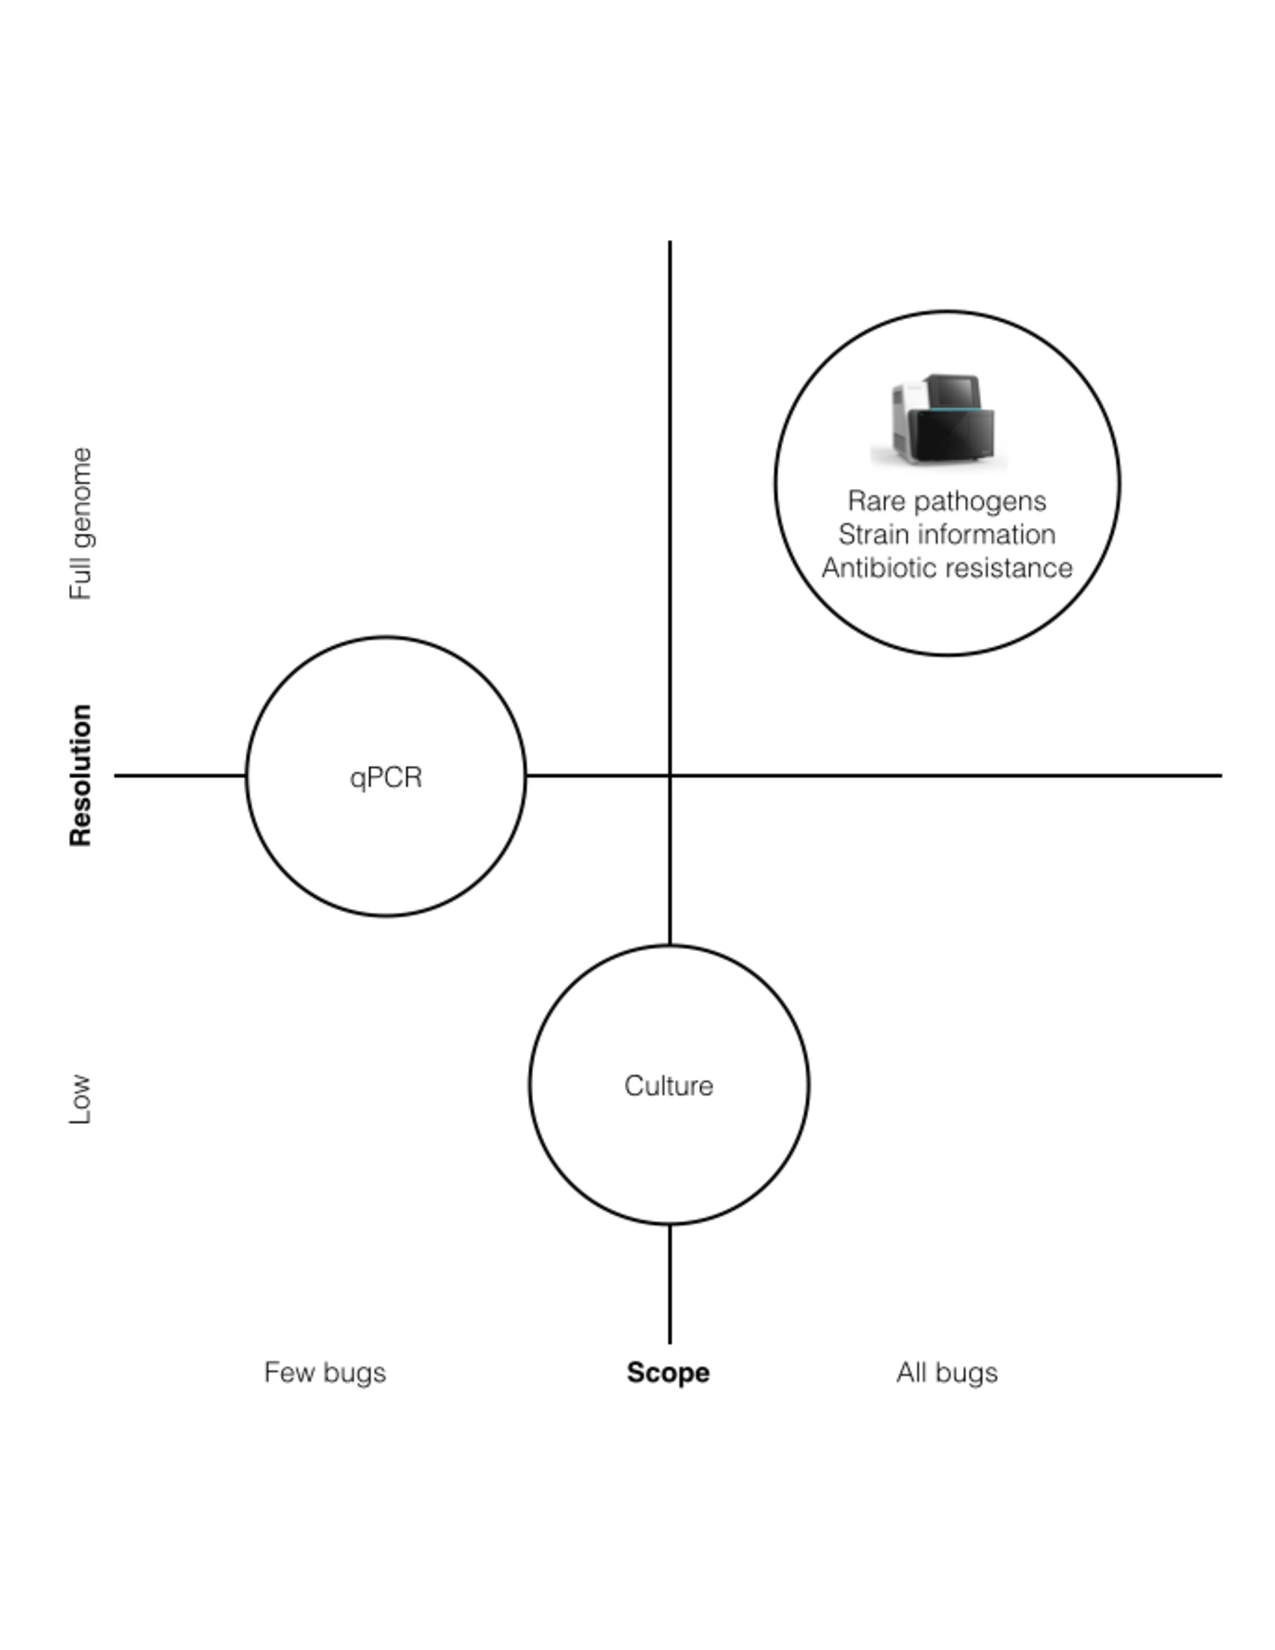
\includegraphics[width=125mm,scale=0.5]{Figures/Fig2}
\caption{The trade-off between scope and resolution.}
\label{fig:Fig2}
\end{figure*}

\subsection{High-throughput methods}

The traditional microbiology lab methods for detecting and identifying bacterial pathogens include Gram staining, solid or liquid culture, the use of the live microbes in tests of biochemical activities and antibiotic resistance, and targeted molecular testing. For most common pathogenic bacteria in humans, these methods are effective, but unusual or novel species can prove difficult to characterize \cite{Boyd:2013cc}. A new era of pathogen identification can be considered to have begun, prior to the availability of HTS methods, with the rapid identification of the SARS virus in 2003, which was achieved through a combination of viral nucleic acid microarray hybridization and traditional viral culture and real-time PCR, followed by sequencing \cite{Boyd:2013cc}.

MALDI-TOF mass spectrometers have become commercialized in order to better address the trade-off between resolution and scope. By identifying proteins with specific signature patterns in a clinical sample and comparing these signatures  to a collection of patterns that have been deposited in a database, MALDI-TOF can achieve better resolution and faster turn-around time than culture-based methods \cite{Fox:2014fj}. Yet, the discriminatory power of the method varies depending on the species and the exhaustiveness of the database used. Some bacterial taxa are under-represented in MALDI-TOF databases, technical problems (such as variations in culture conditions, sample preparation and the spectrometer used) can affect the discriminatory power, and many commercially available databases do not include viruses. 

Soon after the historic publication of the Sanger-sequenced Human Genome Project?s draft results in 2001 and the ?finished? euchromatin sequence in 2004, several new DNA sequencing technologies were described in the literature. Most use a solid flow-cell surface or beads in an emulsion of aqueous droplets in oil to spatially segregate individual DNA template molecules so that they can be amplified in situ, then sequenced with simultaneous data acquisition in parallel from millions of templates via optical or electronic detection.

With these challenges in mind, next-generation DNA sequencing (NGS) has become a very appealing clinical alternative or supplement to MALDI-TOF, culture, or targeted DNA-based methods like qPCR. There are numerous NGS platforms, though all read a large population of amplified DNA fragments in parallel, producing thousands or millions of sequences concurrently \cite{Shendure:2012et}. The critical advantage of NGS in for infectious diseases is that it can, in principle, assay every gene and every conceivable marker derived from infectious agents in a sample. Whereas MALDI-TOF MS relies on a handful of signature proteins, NGS is capable of identifying an unlimited set of possible pathogens (unlimited scope) as well as the complete genomic sequence of each one (high resolution) (Figure ~\ref{fig:Fig2}). Specifically, with sufficiently long read lengths, multiple hits to the microbial genome, and a well-annotated reference database, nearly all microorganisms can be uniquely identified on the basis of their specific nucleic acid sequence. 

\subsection{The case for high-throughput sequencing}

There is great interest in the use of unbiased (NGS) technology for comprehensive detection of pathogens from clinical samples. Conventional diagnostic testing for pathogens is narrow in scope and fails to detect the etiologic agent in a significant percentage of cases  \cite{Naccache:2014gk,}. Failure to accurately diagnose and treat infection in a timely fashion contributes to continued transmission and increased mortality in hospitalized patients. Emergence of novel pathogens further un-derscores the need for rapid, broad-spectrum diagnostic assays that are able to recognize these emerging agents. Several specific studies further highlight this.

\textbf{Unbiased screening of rare pathogens}: Because NGS samples all nucleic acids in a clinical sample in an unbiased fashion, it can reveal infectious causes of illness that escape conventional clinical testing. A recent study applied NGS to a 14-year-old boy with severe combined immunodeficiency that presented with fever and headache that progressed to hydrocephalus and status epilepticus. Though diagnostic workup including brain biopsy were unrevealing, unbiased next-generation sequencing of the cerebrospinal fluid identified an exotic pathogenic bacteria, leptospira. Conventional clinical assays for leptospirosis were negative, though detection with NGS informed intervention and the patient to make a full recovery  \cite{Wilson:2014dv}. 

\textbf{Outbreaks}: Microbiologists and physicians often need to look broadly before determining the virulence genes in a particular strain account for an outbreak. NGS facilitates this search. For example, NGS was used to identify a novel strain of Escherichia coli O157 during a foodborne outbreak in Germany \cite{Fox:2014fj}. US epidemic of community- associated methicillin-resistant Staphylococcus aureus, which found that most strains in different regions of the United States were very closely related; this finding implicates expansion from a single population rather than convergent evolution of different strains  \cite{Boyd:2013cc}. Haitian cholera outbreaks that traced their probable origin to Bangladesh, as well as from an analysis of a particularly virulent Shiga toxin?producing Escherichia coli O104:H4 strain in Germany, which revealed that the en- hanced virulence probably arose by horizontal transfer of a prophage carrying genes for Shiga toxin 2, other virulence factors, and antibiotic resistance.

\textbf{Resistance}: Whole genome sequencing can being used to determine whether plasmids or other mobile genetic elements carrying antimicrobial drug-resistance genes are being transferred among the bacterial pathogens infecting patients. The NIH recently experienced an outbreak of carbapenem-resistant K. pneumoniae that affected 18 patients, 11 of whom died. Integrated genomic and epidemiological analysis traced the outbreak to three independent transmissions from a single patient who was discharged 3 weeks before the next case became clinically apparent and pointed to possible explanations for these transmissions \cite{Fox:2014fj}. In patients who are infected with HIV, deep sequencing of viral subpopulations detects low-frequency mutant viral strains with antivi- ral resistance?associated sequence changes

\textbf{Culture-free}: NGS is valuable in clinical settings when dealing with difficult-to-culture or notoriously slow-growing pathogens such as Mycobacterium tuberculosis.

\textbf{Microbial populations}: NGS can be used to explore microbial diversity at unprecedented depth. We now know that nine Mycobacterium species can cause tuberculosis, some of which, such as Mycobacterium bovis, require specific antibiotic treatments \cite{Fox:2014fj} Furthermore, the human microbiome project has shown that changes in the composition of microbial populations can drive disease \cite{Consortium:2012bb}.

\subsection{NGS challenges and opportunities}

\textbf{Cost and speed}: The cost and turn-around time for sequencing have been driven down by hardware advances. As a result, the cost for determining individual microbial genomes continue to fall (and now cost as little as \$100 per sequence) \cite{Fox:2014fj} with multi-hour turn-around. Both will continue to improve. The justification for NGS will become increasingly apparent, starting with hospital patients who develop difficult-to-treat or life-threatening infections that already prove very costly to the system.

\textbf{Informatics}: NGS provides large datasets that require extensive bioinformatics for sequence analysis, from assembly to annotation. Furthermore, data presentation and distillation of clinical action are highly challenging. Because of the wide spectrum of microbiology labs in terms of technical sophistication, addressing the informatic challenges associated with NGS will be critical for widespread adoption of the technology.
 
\textbf{Mechanism}: Increasingly, NGS has been use to measure the molecular networks that underlie cells, including chromatin immunoprecipitation with subsequent high-throughput sequence analysis (ChIP-Seq) for protein-DNA interactions, high-throughput RNA sequencing (RNA-Seq) for transcription and ?Ribo-Seq? for translation) or even molecular biophysics (for example, parallel analysis of RNA structure (PARS), and global mapping of DNA-DNA interactions using proximity ligation coupled with deep sequencing (Hi-C). Such methods could - in principle - also be applied to infectious disease. 

With these applications in mind, it is a very exciting time for NGS. The MiSeqDX instrument has recently become the first next-generation sequencer approved by the FDA, opening the door for routine implementation of NGS-based assays in the clinical laboratory 

\section{Contributions and outline of this thesis}

(1) NGS can be used to isolate infection-derived DNA fragments can be detected in human blood. (2) These measurements are clinically useful.
(3) Applications can be used to manage this information. (4) NGS can also be used to understand mechanism.
